\section{Security Analysis}
\label{sec:security}

\subsection{Threat Model}

We consider adversaries with the following capabilities:

\begin{enumerate}
    \item \textbf{Malicious Miners}: Control GPU hardware, attempt double-spend
    \item \textbf{Network Attackers}: Observe and manipulate network traffic
    \item \textbf{Quantum Adversaries}: Future quantum computers attacking signatures
    \item \textbf{Colluding Validators}: Up to $f < n/3$ Byzantine validators
\end{enumerate}

\subsection{Quantum Safety}

\subsubsection{ML-DSA Signatures}

All mining signatures use ML-DSA (FIPS 204), providing NIST Level 3 security:

\begin{center}
\begin{tabular}{lccc}
\toprule
\textbf{Algorithm} & \textbf{Classical} & \textbf{Quantum} & \textbf{Key Size} \\
\midrule
ECDSA (current) & 128-bit & $\sim$64-bit & 33 bytes \\
ML-DSA-65 & 192-bit & 128-bit & 1,952 bytes \\
\bottomrule
\end{tabular}
\end{center}

\begin{theorem}[Quantum Resistance]
Under the Module-LWE hardness assumption, ML-DSA signatures are existentially unforgeable under chosen-message attack with quantum adversaries.
\end{theorem}

\subsubsection{Quantum Timeline}

\begin{center}
\begin{tabular}{lcc}
\toprule
\textbf{Year} & \textbf{Threat Level} & \textbf{Mitigation} \\
\midrule
2024--2026 & Low & ML-DSA optional \\
2026--2028 & Medium & ML-DSA default \\
2030+ & High & ECDSA deprecated \\
\bottomrule
\end{tabular}
\end{center}

\subsection{Double-Spend Prevention}

\subsubsection{Spent Set Security}

\begin{lemma}[Spent Set Collision Resistance]
The probability of two distinct work units having the same work ID is:
\begin{equation}
P(\text{collision}) \leq \frac{q^2}{2^{257}} \approx 0
\end{equation}
where $q$ is the number of work units and we use 256-bit BLAKE3.
\end{lemma}

\subsubsection{Chain Binding Security}

\begin{theorem}[Chain Binding Unforgeability]
An adversary cannot produce a valid receipt for chain $C_2$ from work performed for chain $C_1$:
\begin{equation}
\text{Adv}_{\text{forge}}^{\text{chain-bind}}(\mathcal{A}) \leq \text{Adv}_{\text{forge}}^{\text{NVTrust}}(\mathcal{A}) + \text{negl}(\lambda)
\end{equation}
\end{theorem}

\begin{proof}
Chain ID is included in the NVTrust-signed receipt. Modifying the chain ID invalidates the signature. Creating a new valid signature requires breaking NVTrust attestation security.
\end{proof}

\subsection{NVTrust Security}

\subsubsection{Trust Assumptions}

\begin{enumerate}
    \item NVIDIA root CA is trusted and not compromised
    \item GPU firmware is correctly implemented
    \item SPDM protocol is secure against replay and modification
    \item Hardware attestation keys are protected by GPU TEE
\end{enumerate}

\subsubsection{Attestation Chain}

\begin{center}
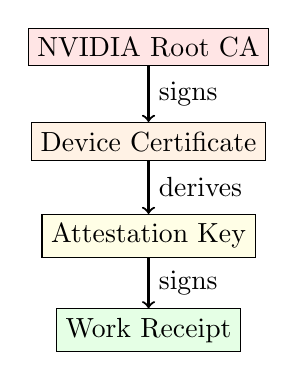
\begin{tikzpicture}[scale=0.8]
    \node[draw, rectangle, fill=red!10] (nvidia) at (0,3) {NVIDIA Root CA};
    \node[draw, rectangle, fill=orange!10] (device) at (0,1.5) {Device Certificate};
    \node[draw, rectangle, fill=yellow!10] (att) at (0,0) {Attestation Key};
    \node[draw, rectangle, fill=green!10] (receipt) at (0,-1.5) {Work Receipt};

    \draw[->, thick] (nvidia) -- node[right] {signs} (device);
    \draw[->, thick] (device) -- node[right] {derives} (att);
    \draw[->, thick] (att) -- node[right] {signs} (receipt);
\end{tikzpicture}
\end{center}

\subsection{Consensus Security}

\subsubsection{Quasar BFT Guarantees}

With $n$ validators and $f < n/3$ Byzantine:

\begin{property}[Safety]
No two honest validators finalize conflicting blocks:
\begin{equation}
\forall v_1, v_2 \in \text{Honest}: \text{finalized}(v_1) \cap \text{finalized}(v_2) \text{ is consistent}
\end{equation}
\end{property}

\begin{property}[Liveness]
If $\geq 2n/3$ validators are honest and network is synchronous, blocks finalize:
\begin{equation}
\forall \text{tx}: \exists t: \text{finalized}(\text{tx}) \text{ by time } t
\end{equation}
\end{property}

\subsection{Teleport Security}

\subsubsection{MPC Security}

Teleport uses CGGMP20 threshold ECDSA with $t$-of-$n$ security:

\begin{theorem}[Threshold Security]
The combined private key is never reconstructed. At least $t$ parties must collude to sign.
\end{theorem}

\subsubsection{Replay Protection}

Each transfer has a unique ID:
\begin{equation}
\text{teleport\_id} = \text{BLAKE3}(\text{source} \| \text{dest} \| \text{sender} \| \text{amount} \| \text{nonce})
\end{equation}

\subsection{Economic Security}

\subsubsection{Mining Attacks}

\begin{center}
\begin{tabular}{lcc}
\toprule
\textbf{Attack} & \textbf{Cost} & \textbf{Mitigation} \\
\midrule
Double-spend & NVTrust break & Hardware attestation \\
Selfish mining & Opportunity cost & Instant finality \\
Empty blocks & No reward & Work requirement \\
\bottomrule
\end{tabular}
\end{center}

\subsubsection{Slashing Conditions}

Misbehaving providers lose stake:

\begin{center}
\begin{tabular}{lc}
\toprule
\textbf{Violation} & \textbf{Penalty} \\
\midrule
Invalid compute result & 10\% stake \\
Timeout / no response & 10\% stake \\
Attestation fraud & 100\% stake \\
Double-sign & 100\% stake \\
\bottomrule
\end{tabular}
\end{center}

\subsection{Key Zeroization}

All secret keys are zeroized on drop:

\begin{lstlisting}[style=rust]
#[derive(Zeroize, ZeroizeOnDrop)]
pub struct SecretKey(Vec<u8>);

impl Drop for SecretKey {
    fn drop(&mut self) {
        self.0.zeroize();
    }
}
\end{lstlisting}

\subsection{Audit Status}

\begin{center}
\begin{tabular}{lcc}
\toprule
\textbf{Component} & \textbf{Auditor} & \textbf{Status} \\
\midrule
Smart Contracts & TBD & Pending \\
ML-DSA Implementation & TBD & Pending \\
NVTrust Integration & TBD & Pending \\
Teleport Protocol & TBD & Pending \\
\bottomrule
\end{tabular}
\end{center}
